% IEEE standard conference template; to be used with:
%   spconf.sty  - LaTeX style file, and
%   IEEEbib.bst - IEEE bibliography style file.
% --------------------------------------------------------------------------

\documentclass[letterpaper]{article}
\usepackage{spconf,amsmath,amssymb,graphicx,float,enumitem,url,algpseudocode}

% Example definitions.
% --------------------
% nice symbols for real and complex numbers
\newcommand{\R}[0]{\mathbb{R}}
\newcommand{\C}[0]{\mathbb{C}}

% bold paragraph titles
\newcommand{\mypar}[1]{{\bf #1.}}

% Title.
% ------
\title{Optimization and parallelization of diffusion solvers\\
using alternating direction implicit and random walk methods}
%
% Single address.
% ---------------
\name{Samuel Maloney} 
\address{Department of Mathematics\\ETH Z\"urich\\Z\"urich, Switzerland}

% For example:
% ------------
%\address{School\\
%		 Department\\
%		 Address}
%
% Two addresses (uncomment and modify for two-address case).
% ----------------------------------------------------------
%\twoauthors
%  {A. Author-one, B. Author-two\sthanks{Thanks to XYZ agency for funding.}}
%		 {School A-B\\
%		 Department A-B\\
%		 Address A-B}
%  {C. Author-three, D. Author-four\sthanks{The fourth author performed the work
%		 while at ...}}
%		 {School C-D\\
%		 Department C-D\\
%		 Address C-D}
%

\begin{document}
%\ninept
%
\maketitle
%


% ----------------------------------------------------------------------
\begin{abstract}
Optimized and parallelized code for numerical simulation of the diffusion equation is presented. Two different algorithms, Alternating Direction Implicit (ADI) and Random Walk (RW) are studied. The algorithms are implemented in C++ and verified against an analytic solution, and then scalar optimizations, AVX vectorization, and OpenMP parallelization are carried out. Benchmarking tests are conducted on the Piz Daint cluster to determine single-core performance and runtime improvements, as well as strong and weak scaling characteristics on multiple cores of a single node. Approximate performance gain of 5X for ADI, and runtime speedups of approximately 6X and 3000X for ADI and RW respectively are observed, along with acceptable OpenMP scaling.
\end{abstract}


% ----------------------------------------------------------------------
\section{Background}\label{sec:background}

\mypar{Motivation} 
Diffusion is the process by which a~quantity of interest spreads from regions of high density to regions of low density and are integral in the study of fluids. Diffusion terms arise in all numerical models of computational fluid dynamics, which are used for such problems as aerodynamic design, turbine flows, chemical reaction mixing, and many others. Efficient and accurate simulation codes for diffusion are thus of great importance in many fields.

In this study, two different algorithms to simulate the diffusion process, Alternating Direction Implicit (ADI) and Random Walk (RW), were implemented, optimized, and parallelized. The mathematical formulations for diffusion in general and for each of these two methods specifically are presented next.

\mypar{Mathematical Formulation}
The process of diffusion is driven by it's conentration gradient according to the diffusion equation:
\begin{equation}
\frac{\partial \rho(\mathbf{r},t)}{\partial t} = D\Delta\rho(\mathbf{r},t)
\label{diff}
\end{equation}
where $\rho(\mathbf{r},t)$, with position $\mathbf{r}$ at time $t$, is the quantity of interest and $D$ is the diffusion constant and is a given value for the system. For this study, homogeneous Dirichlet boundary conditions are used at all boundaries. The initial density distribution used for this study is:
\begin{equation}
\rho(x,y,0)=\sin(\pi x)\sin(\pi y)
\end{equation}
and it's corresponding analytic solution, which was used for verification, is:
\begin{equation}
\rho(x,y,t)=\sin(\pi x)\sin(\pi y)e^{-2D\pi^{2}t}
\label{analytic}
\end{equation}
The studied simulation domain is a unit square with $x$ and $y$ each ranging from $0$ to $1$, which is discretized using a uniform grid such that $\delta h=\delta x=\delta y$. A superscript $n$ is used to denote the timestep $t_n=n\delta t$ and subscripts $i$ and $j$ to denote the indices of the nodes in the mesh $x_i=i\delta x$ and $y_j=j\delta y$ such that $\rho_{i,j}^{n}=\rho(x_i,y_j,t_n)$.

\mypar{Alternating Direction Implicit}
The ADI method is an operator splitting scheme based on finite difference discretizations of the derivatives. It works by splitting the each time step into two half tiem steps, in the first of which the time integration is carried out implicitly in the $x$-direction and explicitly in the $y$-direction, and in the second half time step the directions are switched such that the integration in the $x$-direction is explicit and in the $y$-direction is implicit.

Using a second order centered approximation for the spatial derivative in Eq. \eqref{diff} means that each implicit integration step requires only the solution of a tridiagonal linear system, for which the Thomas Algorithm (for formulation see \cite{thomas}) can be used to efficiently compute the result. These tridiagonal systems can be found by considering the discretization equations:
\begin{equation}
\rho_{i,j}^{n+\frac{1}{2}}=\rho_{i,j}^n+\frac{D\delta t}{d\delta x^2}(\rho_{i-1,j}^{n+\frac{1}{2}}-2\rho_{i,j}^{n+\frac{1}{2}}+\rho_{i+1,j}^{n+\frac{1}{2}})
\end{equation}
\begin{equation}
\rho_{i,j}^{n+1}=\rho_{i,j}^{n+\frac{1}{2}}+\frac{D\delta t}{d\delta x^2}(\rho_{i,j-1}^{n+1}-2\rho_{i,j}^{n+1}+\rho_{i,j+1}^{n+1})
\end{equation}
These can be rewritten in the form $\mathbf{A}\rho^*=\rho^{*-\frac{1}{2}}$ where $\mathbf{A}$ is the tridiagonal matrix to be solved at each half timestep.

\mypar{Random Walk}
Diffusion can also be simulated by tracking the random motion of a set of $M$ identical particles with no inertia. A probability $\lambda=D\delta t/\delta x^2$ is defined, such that at each time step, each particle has a $1-4\lambda$ probability of remaining in the same position. If it does not stay, it is then moved to one of the 4 neighbouring nodes, with an equal probability of moving in any direction. Clearly, one requires $lambda<1/2$ to maintain a positive probability of staying.

The initial conidition for the numer of particles at each grid point $m_{i,j}$ is given as:
\begin{equation}
m_{i,j}^0=\left \lfloor{\frac{M\rho(x_i,y_j,0)}{\iint_\Omega \rho(x,y,0) \,\mathrm{d}x\,\mathrm{d}y}}\right \rfloor 
\end{equation}
And the approximate solution after a given timestep can then be calculated as:
\begin{equation}
\rho_{i,j}^n=\frac{m_{i,j}^n}{M}\iint_\Omega \rho(x,y,0)  \,\mathrm{d}x\,\mathrm{d}y
\end{equation}

% ----------------------------------------------------------------------
\section{Baseline Implementation}\label{sec:baseline}

In this section, the basic implementation and verification of the described algorithms is presented. All code is based on the Diffusion2D class structure of the solution code provided with the course exercises. All code for each version of the class is contained within a single .cpp source file, and includes user defined header files \textit{timer.hpp} and \textit{tsc\_x86.hpp} for measuring runtime in seconds and cycles respectively. The \textit{timer.hpp} file is from the HPCSE I course exercises, and the \textit{tsc\_x86.hpp} file is from the exercises of the How to Write Fast Numerical Code course exercises.

The programs take arguments to set the diffusion constant $D$, size $N$ of one dimension of the grid, timestep $\delta t$, number of repititions $n_{runs}$ to run the simulation, and the number of timesteps $n_{steps}$ to run each simulation for. The RW codes also take a value for the numer of particles $M$ in the simulation. For all codes the values for $n_{runs}$ and $n_{steps}$ are optional, and default to $n_{runs}=1$ and $n_{steps}=0.1/\delta t$ respectively. The ordering of these input arguments can be displayed by running the program with no arguments.

For each simulation run, a new Diffusion2D class object is initialized, with one-time initialization routines happening outside of the timing structures. Once initialization is complete, the simulation is is run to completion by a single call to the {\tt run\_simulation} function, and this call is the only part of the program which is timed and contains all code which will be optimized. 

\mypar{ADI}
An order verification study (OVS) of the ADI code in both spatial and temporal diensions was performed by comparing the simulation results to the analytic solution in Eq. \eqref{analytic}. The results can be seen in Fig. \ref{fig:OVS_ADI} and show the implementation to be second order accurate in both space and time, as expected for this discretization scheme.

The ADI algorithm complexity should be $O(N^2)$ as it does a constant number of operations for updating value at each point in the grid. It's runtime scaling (see \ref{subsec:ADI_results}, Fig. \ref{fig:runtime_ADI}) is also found to agree with this expected complexity.

\begin{figure}\centering
  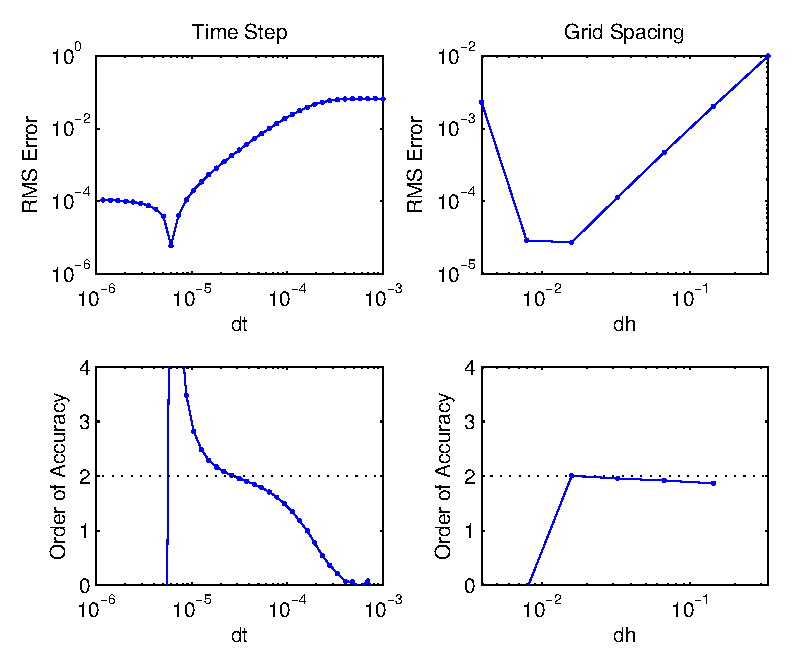
\includegraphics[width=\linewidth]{./plots/OVS_ADI_cropped.eps}
  \caption{Order Verification study of the ADI code.}
  \label{fig:OVS_ADI}
\end{figure}

For performance analysis, the cost of the ADI code is defined as the number of floating point operations (FLOPs) including additions, multiplications, and, for the baseline implementation only, divisions. Moreover, the data movement in bytes between various levels of cache was measured using the Hardware Performance Counter (HWPC) functionality in CrayPat to quantify the operational intensity.

The results of a roofline analysis are shown in Fig. \ref{fig:roofline_ADI_serial} for the baseline code. Three data series are presented, which use the same performance data but compute the operational intensity with respect to different levels of the cache heirarchy. The imlementation appears compute bound with respect to memory tranfers with RAM, but for large $N$ it becomes clearly memory bound at higher levels of the cache, albeit with still siginificant room to improve towards the memory bandwidth rooflines. Maximum performance of 0.734 FLOPs/cycle, or 18\% of peak scalar performance is observed. On the test machine, with an Intel Haswell central processing unit (CPU), the peak performance is calculated by considering the maximum throughput of 2 fused multiply add (FMA) instructions per cycle, giving 4 total FLOPs per cycle. Data for the cache bandwidths used in this (and subsequent) roofline plots was obtained from \cite{7_cpu} and \cite{manual_intel}.

\mypar{RW}
Lorem Ipsum dolor sit amet.

\begin{figure}\centering
  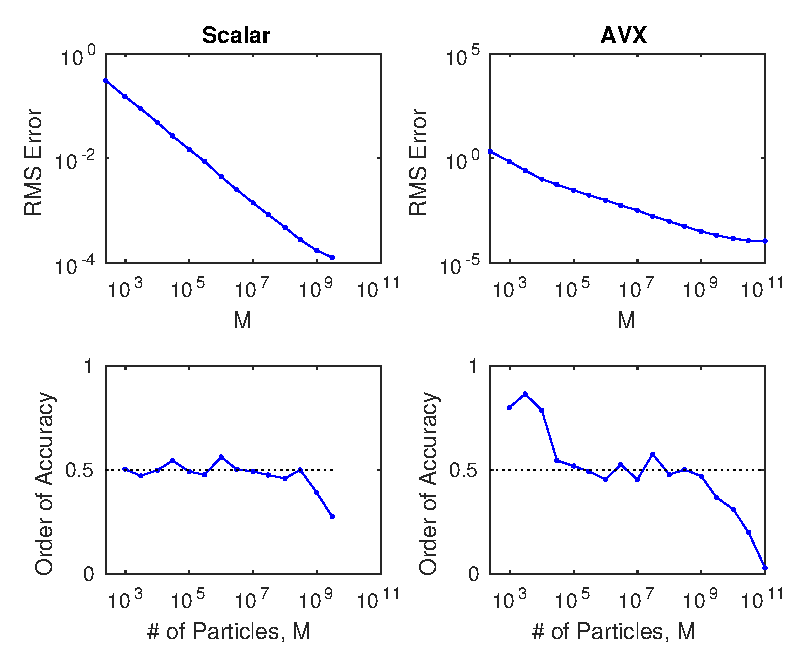
\includegraphics[width=\linewidth]{./plots/OVS_RW_cropped.eps}
  \caption{Order Verification study of the RW code.}
  \label{fig:OVS_RW}
\end{figure}

Scaling for the RW method depends on which version is being considered. The baseline implementation should scale as $O(M)$, where $M$ is the number of particles in the simulation. This is because a random number must be generated for each particle in the simulation to determine it's movement for a given timestep, independent of how many grid points there are in the simulation. The later versions that use a binomial random variable (see \ref{subsec:RW_method}) to simulate particle movement scale as $O(N^2)$ because exactly four such random variables must be evaluated for each grid point, independent of the number of particles in the simulation.


% ----------------------------------------------------------------------
\section{Optimization Method}\label{sec:method}

In this section we explain the main optimizations that were undertaken.
We discuss the optimizations of the ADI and RW methods in separate subsections.

\subsection{ADI}\label{subsec:ADI_method}

We divide the optimizations in 4 sets called \textit{revisions}.

\mypar{Scalar}
This revision consists mainly of 

\mypar{AVX}
In this revision we used

\mypar{OpenMP}
This revision was targeted at 


\subsection{RW}\label{subsec:RW_method}

TheRW optimizations can be similarly broken down into revisions, simlarily to those for the assembly.

\mypar{Scalar}
This is a direct implentation

\mypar{AVX}
Vectorization of the code was done by leveraging Intel fused-multiply-add (FMA) and advanced vector extension (AVX) intrinsics.

\mypar{OpenMP}
stuff...


% ----------------------------------------------------------------------
\section{Optimization Results}\label{sec:results}

In this section the results of numerical benchmarks of the code at various stages are presented. Runtime, performance, and roofline analyses were performed where applicable.

\mypar{Experimental setup}
All data was collected using a single XC50 node of Piz Daint, which has a 12 core Intel Xeon E5-2690 v3 running at 2.6 GHz \cite{daint}. Each physical processor core has a 64 KB L1 cache split equally into two 32 KB data and instruction caches, and a 256 KB unified L2 cache \cite{cpu_world}. The 30 MB L3 cache is shared between all cores \cite{ark_intel}, and there is 24.9 GB/s bandwidth to main memory \cite{7_cpu}. The Intel C++ Compiler v17.0.1 was used with "-O3 -std=c++11 -DNDEBUG -march=core-avx2 -fno-alias -qopenmp -mkl" flags. The Intel time stamp counter (TSC) was used for runtime measurements and CrayPat was used for cache miss measurements.

The inputs are the number of grid points in domain discretization, the timestep between iterations, and the number of timesteps computed. We used grids of various sizes, up to $N\times N=7680\times7680$. The diffusion constant $D=1$ is used for all simulations, and for RW simulations $M=1000N^2$ particles were used. For ADI, $1000$ iterations were performed, and for RW $50$ iterations were performed to achieve a reasonable runtime for measurements. Each simulation was repeated $10$ times, with the minimum cycle count used for the runtime and the average cache misses used for the memory transfer (the average is used only because it would have prohibitively time-consuming to measure minimum values with CrayPat).

All experiments were performed with warm cache. This is largely to simulate real world usage scenarios, where the simulation would most likely be performed immediately after initialization while the data is still potentially in cache, exactly as in these experiments. It is noted, however, that the initial cache state should have little effect on the results in either case, as the effects will be amortized over the number of iterations performed, and should become negligible for the relatively large number of iterations used.

\subsection{ADI}\label{subsec:ADI_results}
Roofline, runtime, and scaling experiments were conducted on the ADI code.

\mypar{Results}
The runtime plots of various revisions of the ADI code (see \ref{subsec:ADI_method}) are shown in Fig. \ref{fig:runtime_assemby}. Each consecutive revision of the code resulted in a~speedup.

\begin{figure}\centering
  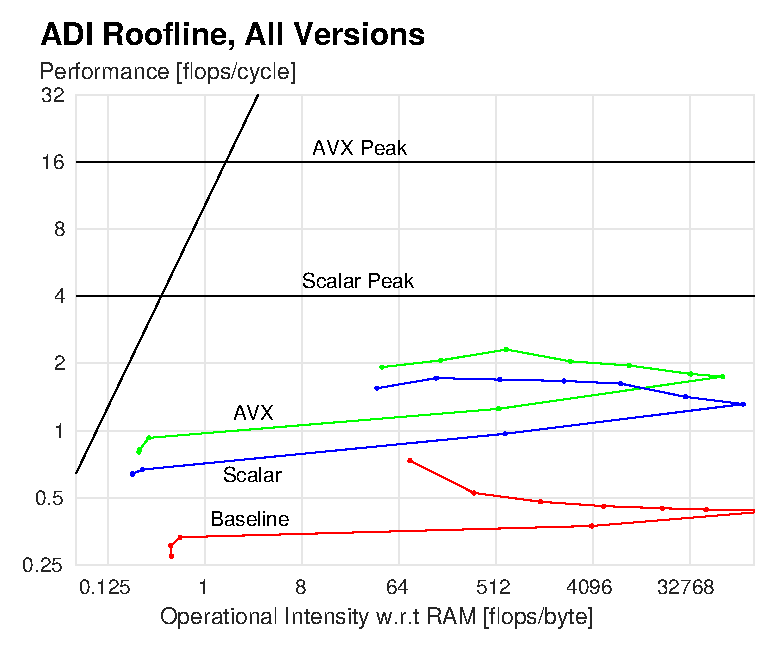
\includegraphics[width=\linewidth]{./plots/roofline_ADI_all_cropped.eps}
  \caption{Roofline analysis of the ADI code.}
  \label{fig:roofline_ADI_all}
\end{figure}

\begin{figure}\centering
  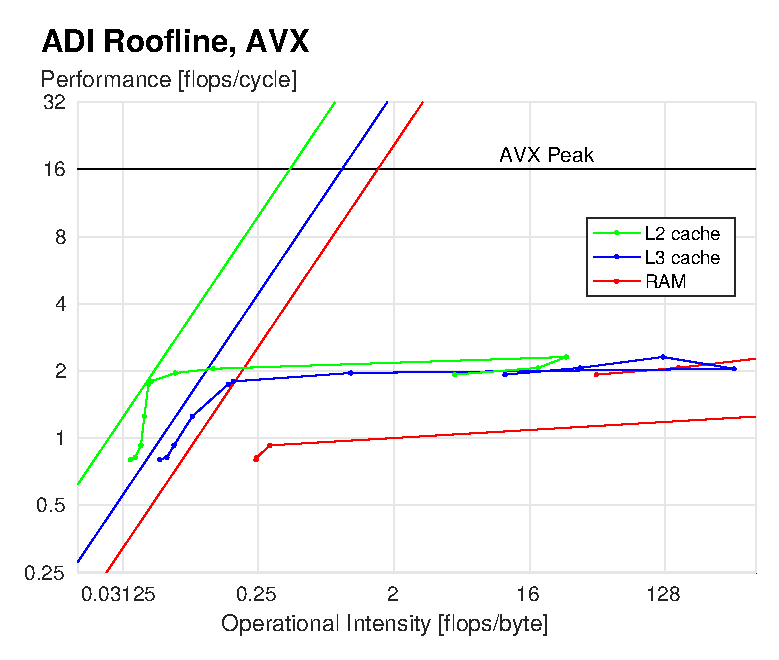
\includegraphics[width=\linewidth]{./plots/roofline_ADI_AVX_cropped.eps}
  \caption{Roofline analysis of the ADI AVX code.}
  \label{fig:roofline_ADI_AVX}
\end{figure}

\begin{figure}\centering
  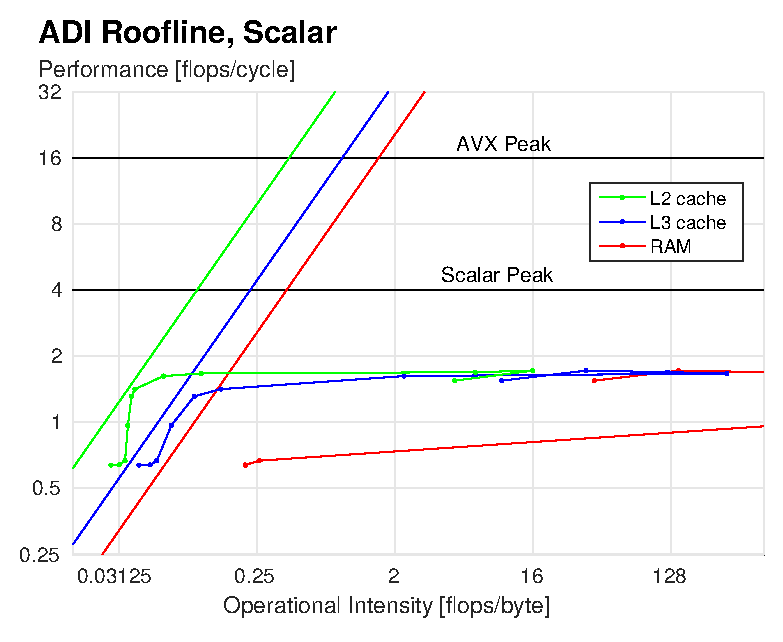
\includegraphics[width=\linewidth]{./plots/roofline_ADI_scalar_cropped.eps}
  \caption{Roofline analysis of the ADI scalar code.}
  \label{fig:roofline_ADI_scalar}
\end{figure}

\begin{figure}\centering
  \includegraphics[width=\linewidth]{./plots/runtime_ADI_cropped.eps}
  \caption{Runtime analysis of the ADI code.}
  \label{fig:runtime_ADI}
\end{figure}

\begin{figure}\centering
  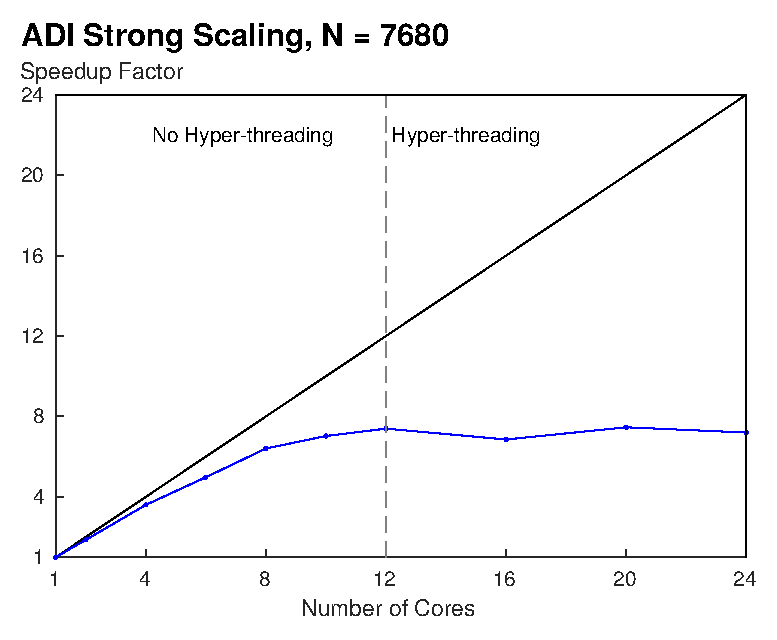
\includegraphics[width=\linewidth]{./plots/scaling_strong_ADI_cropped.eps}
  \caption{Strong Scaling analysis of the ADI OpenMP code.}
  \label{fig:scaling_strong_ADI}
\end{figure}

\begin{figure}\centering
  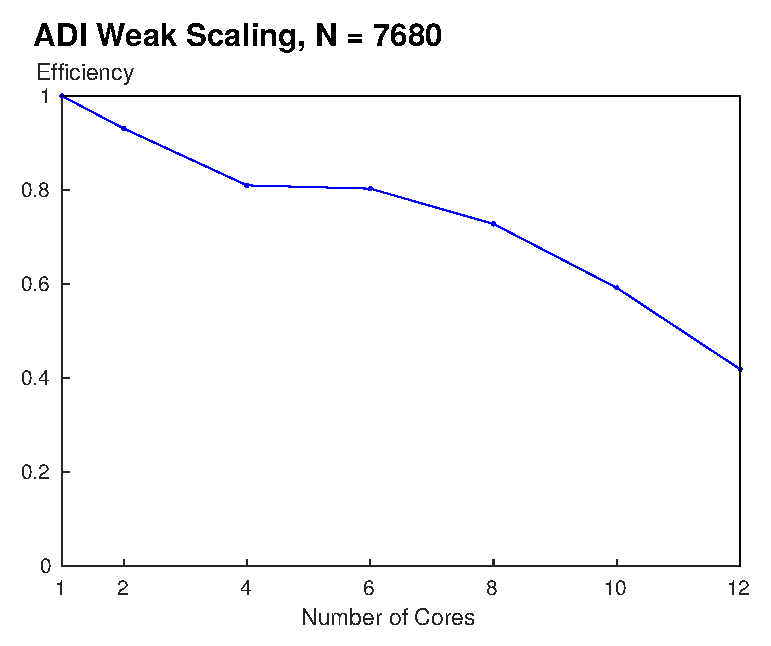
\includegraphics[width=\linewidth]{./plots/scaling_weak_ADI_cropped.eps}
  \caption{Weak Scaling analysis of the ADI OpenMP code.}
  \label{fig:scaling_weak_ADI}
\end{figure}

\subsection{RW}\label{subsec:RW_results}
Benchmarking experiments were conducted on the RW code

\mypar{Results}
Results of the roofline, performance, and runtime analyses of the RW code will now be presented.

\begin{figure}\centering
  \includegraphics[width=\linewidth]{./plots/runtime_RW_cropped.eps}
  \caption{Runtime analysis of the RW code.}
  \label{fig:runtime_RW}
\end{figure}

\begin{figure}\centering
  \includegraphics[width=\linewidth]{./plots/scaling_strong_RW_cropped.eps}
  \caption{Strong Scaling analysis of the RW OpenMP code.}
  \label{fig:scaling_strong_RW}
\end{figure}

\begin{figure}\centering
  \includegraphics[width=\linewidth]{./plots/scaling_weak_RW_cropped.eps}
  \caption{Weak Scaling analysis of the RW OpenMP code.}
  \label{fig:scaling_weak_RW}
\end{figure}


% ----------------------------------------------------------------------
\section{Conclusion}
Conclude things

% ----------------------------------------------------------------------


\begin{thebibliography}{99}

\urlstyle{same}

\bibitem{thomas}{Wikipedia. (2017, May 16). \emph{Tridiagonal matrix algorithm} [Online]. Available: \url{https://en.wikipedia.org/wiki/Tridiagonal_matrix_algorithm}}

\bibitem{daint}{CSCS. (Accessed 2017, Aug). \emph{Piz Daint} [Online]. Available: \url{http://www.cscs.ch/computers/piz_daint/}}

\bibitem{7_cpu}{7-CPU. (Accessed 2017, Aug). \emph{Intel Haswell} [Online]. Available: \url{http://www.7-cpu.com/cpu/Haswell.html}}

\bibitem{manual_intel}{Intel Corporation. (2016, Jun). \emph{Intel 64 and IA-32 Architectures Optimization Reference Manual} [Online]. Available: \url{https://www.intel.com/content/www/us/en/architecture-and-technology/64-ia-32-architectures-optimization-manual.html}}

\bibitem{cpu_world}{CPU-World. (Accessed 2017, Aug). \emph{Intel Xeon E5-2690 v3 specifications} [Online]. Available: \url{http://www.cpu-world.com/CPUs/Xeon/Intel-Xeon%20E5-2690%20v3.html}}

\bibitem{ark_intel}{Intel Corporation. (Accessed 2017, Aug). \emph{Intel Xeon Processor E5-2690 v3} [Online]. Available: \url{http://ark.intel.com/products/81713/Intel-Xeon-Processor-E5-2690-v3-30M-Cache-2_60-GHzl}}

\bibitem{transpose}{user2927848. (2016, Mar 23). \emph{m256d TRANSPOSE4 Equivalent} [Online]. Available: \url{https://stackoverflow.com/questions/36167517/m256d-transpose4-equivalent}}

\bibitem{sitmo}{T. van den Berg. (Accessed 2017, Aug). \emph{High Quality C++ Parallel Random Number Generator} [Online]. Available: \url{https://www.sitmo.com/?p=1206}}

\end{thebibliography}

\end{document}
